\chapter{Simulation framework in EPANET}
\label{simulation_framework_in_EPANET}

\emph{This chapter gives an insight into the simulation model of the Randers WSS in EPANET. In order to understand better how the simulation works, the modelling of the different pumping stations, waterworks, and the consumption patterns are explained in detail. In the end, an attempt is made to split the network into different subsystems and make necessary modifications such that data is sufficiently reduced and therefore easily extractable for system identification purposes.}

% \emph{This chapter gives a general introduction about the need for model simplification in WSSs. Different approaches and methods are discussed in a state of art manner, including the development and methodologies employed in this field. Lastly, an attempt is made to simplify the Randers WSS, using one of the techniques which are being introduced in this chapter. }

\section{Model and data structure}
\label{model_data_and_structure}

As it was explained in \chapref{description_of_water_supply_systems}, the typical components of WSSs are: reservoirs, pipes, pumps and valves. For simulation purposes, it is required that the model of the real-life network consists of thousands of elements in order to accurately replicate hydraulic behaviour and the topographical layout of the system. Such models are appropriate for simulation purposes, however, online optimisation tasks are much more computationally demanding. Therefore the available data in the simulation framework will be used to create a reduced order model for control purposes. 

The use of Geographic Information Systems(GIS) and Supervisory Control  and Data Acquisition(SCADA) systems in the water industry resulted in an increasing amount of information about actual network topology and service that can be utilized in a model \cite{johnson2016geographic}. As a consequence of this, normally the simulation model of WSSs include exactly the same amount of components as in real-life. 

The following data and model description strongly relies on the documentation of the Randers WSS EPANET model \cite{verdo_doc}, provided by Verdo A/S, where the considerations and modelling steps with the available data from GIS are gathered. The model is mainly based on the data stored in GIS and the SCADA system, however considerations on case studies and experience have also been taken into account. It is important to note that the following results and properties of the EPANET model serve as a basis for the data processing and therefore is discussed in the report.  

Initially, during the modelling, nodes were made among each different pipe elements, however this increased the calculation time significantly. Therefore the number of nodes in the network were reduced based on the fact that pipe sections with the same material and dimensions can be treated as one pipeline. In order to illustrate the complexity of the network, the number of elements in the simulation model, including the VSV region, is shown in \tabref{numberofelements_table}

\begin{center}
\label{numberofelements_table}
    \begin{tabular}{ | p{3cm} | p{3cm} |}
    \hline
    \textbf{Element type} & \textbf{Number}  \\ 
    \hline
    Links & 4144  \\ 
    \hline
    Nodes & 4180  \\ 
    \hline
    Tanks & 6  \\ 
    \hline
    \end{tabular}
    \captionof{table}{Number of WSS elements.}
\end{center}

\vspace{-3mm}

When we consider the simulation of the network in EPANET, it needs to be stated that certain abstractions were made in the model. These abstractions are not necessarily reflect the real-world configuration of the system, however with including them in the model, the same results can be achieved as in real-world. Therefore for instance the number of WTs in the model does not necessarily reflect the number of WTs in the real system. Water works usually have large WTs, where the aeration process and filtering is being done, however in some parts water works abstractions are used for water sources, being replaced with nodes. Furthermore, in certain parts of the system, the modelling reflects the real-world. However, the structure of certain pumping stations are different from the real world. For the same reason, at some places in the simulation, one pump serves to simulate a whole pumping station while in the real world more pumps are placed in parallel. 

\subsection{Water consumption data}
\label{water_consumption_data}

In the model, consumption data is divided into two groups: non-industrial and industrial demands. It has been chosen to keep the number of demand categories low, as it turned out that the quality of this data from GIS is not representative. This is due to the fact that single one storey buildings and two or more storey buildings have very similar consumptions. The consumption curves were defined such that they match the pumped water volumes from waterworks and pumping stations in each individual zone. Therefore, a calculation for the deviation has been made over the day such that it was possible to conclude on the uniformity of the consumption types in each zone \cite{verdo_doc}. With around 3 percent uncertainty, the consumption patterns turned out to be reliable in the model. The demand patterns over a 24 hours long period are shown in \figref{fig:demandpatterns_EPANET} .

\begin{figure}[H]
\centering
%
\includegraphics[width=0.4\textwidth]{report/pictures/missingfigure}
% This file was created by matlab2tikz.
%
%The latest updates can be retrieved from
%  http://www.mathworks.com/matlabcentral/fileexchange/22022-matlab2tikz-matlab2tikz
%where you can also make suggestions and rate matlab2tikz.
%
\definecolor{mycolor1}{rgb}{0.00000,0.44700,0.74100}%
\definecolor{mycolor2}{rgb}{0.85000,0.32500,0.09800}%
%
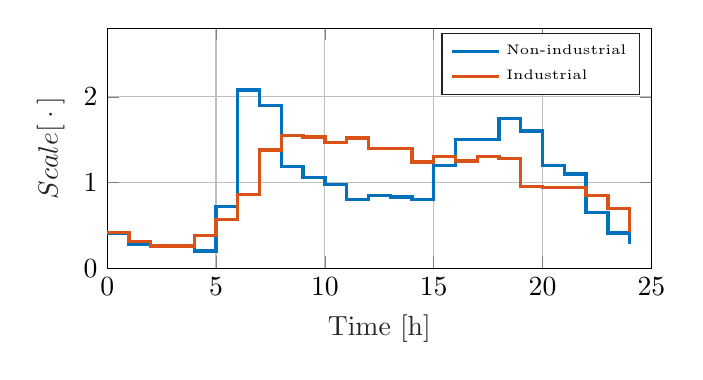
\begin{tikzpicture}

\begin{axis}[%
width=2.721in,
height=1.2in,
at={(0.758in,0.481in)},
scale only axis,
xmin=0,
xmax=25,
xlabel style={font=\color{white!15!black}},
xlabel={Time [h]},
ymin=0,
ymax=2.8,
ylabel style={font=\color{white!15!black}},
ylabel={$\text{Scale [}\cdot\text{]}$},
axis background/.style={fill=white},
%title style={font=\bfseries},
%title={Industrial/non-industrial water consumption pattern},
xmajorgrids,
ymajorgrids,
legend style={legend cell align=left, align=left, draw=white!13!black}
]
\addplot[const plot, color=mycolor1, line width=1.2pt] table[row sep=crcr] {%
0	0.41\\
1	0.280000000000001\\
2	0.25\\
3	0.260000000000002\\
4	0.199999999999999\\
5	0.719999999999999\\
6	2.08\\
7	1.9\\
8	1.19\\
9	1.06\\
10	0.98\\
11	0.800000000000001\\
12	0.850000000000001\\
13	0.829999999999998\\
14	0.800000000000001\\
15	1.2\\
16	1.5\\
18	1.75\\
19	1.6\\
20	1.2\\
21	1.1\\
22	0.649999999999999\\
23	0.41\\
24	0.280000000000001\\
};
\addlegendentry{\tiny Non-industrial}

\addplot[const plot, color=mycolor2, line width=1.2pt] table[row sep=crcr] {%
0	0.420000000000002\\
1	0.309999999999999\\
2	0.260000000000002\\
4	0.379999999999999\\
5	0.57\\
6	0.859999999999999\\
7	1.38\\
8	1.55\\
9	1.53\\
10	1.47\\
11	1.52\\
12	1.4\\
14	1.24\\
15	1.3\\
16	1.25\\
17	1.3\\
18	1.28\\
19	0.949999999999999\\
20	0.940000000000001\\
22	0.850000000000001\\
23	0.699999999999999\\
24	0.420000000000002\\
};
\addlegendentry{\tiny Industrial}

\end{axis}
\end{tikzpicture}%
\caption{Industrial and Non-industrial demand patterns in the EPANET simulation.}
\label{fig:demandpatterns_EPANET}
\end{figure}

\vspace{-3mm}

In \figref{fig:demandpatterns_EPANET}, the $y$-axis shows the ratio of change compared to the base demand of the two different types of consumers. For each type of consumer, different base demands are determined. However, the variation from this base value can be described in the same manner with the presented consumption curves for users falling in the same category. 

It is worth noting that the industrial consumption profile in the VSV zone slightly differs from the industries in the rest of the network. However, since the VSV zone is not considered in the further simulation model, the demand pattern is not shown here. Furthermore, there are no consumers in the corresponding supply areas who have  significant effect on water consumption to influence the model calibration and simulation. 

\subsection{Control and water source abstractions}
\label{control_and_water_source_abstractions}

As described in \secref{the_randers_water_supply_network}, there are several different pumping stations and waterworks in the network, supplying different zones. In general, there is a possibility in EPANET to simulate the cleaning process in the waterworks, including drilling, raw water and clean water treatment. However, in the model the focus is on the correct distribution. Therefore, all waterworks are simulated with clean water reservoirs. In the EPANET simulation, pumps in the waterworks pump the water out corresponding to the real pump curves. However, there are two exceptions, where the simulation of the pumping station is different. In the OMV water work, which is responsible for filling the tanks(T1A and T1B) in HBP pumping station, the precise operation has not been taken into account. Instead, the control schedule of the pumps has been simulated as a positive demand node, which is negative according to the EPANET sign convention. The same technique was used in HBP pumping station, where the two tanks are located and which provides the distribution to the HZ. One of the reasons for this is that the controls turned out to be relatively complicated with frequency converters and the simulation result of the pumping was not matching the real world scenario. The advantage of this is that in one of the flow controlled pumping stations, the mass balance is controlled. Furthermore, the risk that the model does not simulate correctly is reduced. It should be noted that this abstraction can be done easily in HBP and OMV, since pumps in these two pumping stations are flow controlled. 

Apart from the OMV water work and HBP pumping station, all water works have been simulated with reservoirs which cannot be emptied. Water works and pumping stations, where the pumps are pressure controlled, are controlled by PRVs, as this is the typical way of controlling pressure controlled pumps in EPANET networks \cite{agency2016epanet}. Such an arrangement is shown in \figref{fig:PRV_EPANET} 

 %Waterworks in EPANET
\begin{figure}[H]
\centering
%
\includegraphics[width=0.35\textwidth]{report/pictures/missingfigure}
\begin{tikzpicture}[scale=0.6,transform shape]

\begin{scope} [rotate around={0:(12,5.5)}, shift={(0.8,0)}]
\draw[thick,transform shape] (12,5.5) circle (0.5);
\draw[thick,transform shape] (12.5,5.5) -- (12,6);
\draw[thick,transform shape] (12.5,5.5) node (v1) {} -- (12,5);
\end{scope}

%man-valve
\begin{scope} [rotate ={-90}]
\node(n1) at (-5.25,16) {};
\draw[thick,transform shape](n1.center) -- ($(n1)-(0.5,0)$) --
($(n1)-(0,1)$) -- ($(n1)-(0.5,1)$) --  (n1.center);

\end{scope}

\draw [thick](15,5.5) -- (13.3,5.5);
\node at (15.5,6.2) {\large PRV};
\draw [thick](16,5.5) -- (17.5,5.5);
\draw [fill=cyan] [thick](9.1,5.7) -- (9.1,5.1) -- (10.9,5.1) -- (10.9,5.7);
\draw  [thick](9.1,6.1) -- (9.1,5.1) -- (10.9,5.1) -- (10.9,6.1);
\draw [thick](12.3,5.5) -- (10.9,5.5);
\end{tikzpicture} 
\caption{Abstraction for pressure controlled pumping stations in EPANET.}
\label{fig:PRV_EPANET}
\end{figure}

\vspace{-3mm}
It is important to note, however, that in case of high demands, with this arrangement in the network it can happen that water works and pumping stations deliver more flow than allowed or physically possible. Therefore control rules have been incorporated in the models which prevent the pumping stations produce more flow than available in the real world. 

In case of flow controlled pumping stations, such as OMV, the following abstractions are made in the EPANET simulation framework 

 %Flowcontrolled pumping stations in EPANET
\begin{figure}[H]
\centering
%
\includegraphics[width=0.35\textwidth]{report/pictures/missingfigure}
\begin{tikzpicture}[scale=0.65,transform shape]

\draw[fill=black] (10.7,2.2) node (v2) {} circle (.6ex);

\draw[fill=black] (11.9,2.2) node (v1) {} circle (.6ex);
\node at (12.5,3) {\large $d_+$};
\node at (14.5,3) {\large FCV};
\node at (10,3) {\large $d_-$};

\draw [-latex](v1);
\draw [thick](v1) -- (14,2.2);
\draw [thick](v2) -- (9.2,2.2);

\draw[fill=black] (9.1,2.2) node (v1) {} circle (.2ex);
\draw[fill=black] (8.7,2.2) node (v1) {} circle (.2ex);
\draw[fill=black] (8.9,2.2) node (v1) {} circle (.2ex);

\draw [-latex]  (9.4,2.7)--(10.7,2.7);
\draw [-latex](11.9,2.7) -- (13.2,2.7);

%man-valve
\begin{scope} [rotate ={-90}]
\node(n1) at (-1.95,15) {};
\draw[thick,transform shape](n1.center) -- ($(n1)-(0.5,0)$) --
($(n1)-(0,1)$) -- ($(n1)-(0.5,1)$) --  (n1.center);

\end{scope}

\draw [thick](15,2.2) -- (15.8,2.2);
\end{tikzpicture} 
\caption{Abstraction for flow controlled pumping stations in EPANET.}
\label{fig:FCV_EPANET}
\end{figure}

\vspace{-3mm}

In \figref{fig:FCV_EPANET}, the node which has demand $d_+$ is the flow controlled pumping station. The water coming out from this node can be controlled by a FCV. In every case, the pumping stations are supplied by flow from water works. A good example for this is TBP pumping station where the water works BKV and ØSV are modelled. However, the pumping station can be modelled as two nodes, where inflow is defined on the node on the water work side and outflow is defined on the outlet side. 

\section{Model calibration and validation}
\label{model_calibration_and_validation}

The simulation data has been validated by using pressure measurements on different fire hydrants in the network for several times corresponding to different years. When the model was made, the data was not completely up to date, as these pressure measurements were carried out in years before the EPANET modelling. The major uncertainty about this data is in the arrangement of the pipe network and the pumping stations, since it has been changed over the years and old facilities have been replaced. Although the data on which the model relies is uncertain and there might be variations in pressure, the validation of the model has been carried out according to these highly uncertain pressure measurements. 

\subsection{Pipe roughness}
\label{pipe_roughness}

In the model, all pipes are associated with tags, indicating dimensions, material and year information. With this information it is possible to estimate an average resistance, i.e. roughness of the pipes. 
During the validation process of the pipe resistances, it was chosen to consider an average roughness value, taking into account that the roughness should not be lower than a roughness of new pipes and at the same time, should not exceed a certain upper bound. Roughnesses were upscaled at places where the pressure was too high while downscaled where the pressure was certainly too low. Correct pressure data, however is an essential information for a more detailed and precise calibration, therefore high deviations up to 5 meter heads are present in the system. \figref{fig:pressure_mistakes} shows the pressure deviation in the system compared to the data on which the system was calibrated. 

%Fire hydrants measurements
\begin{figure}[H]
\centering
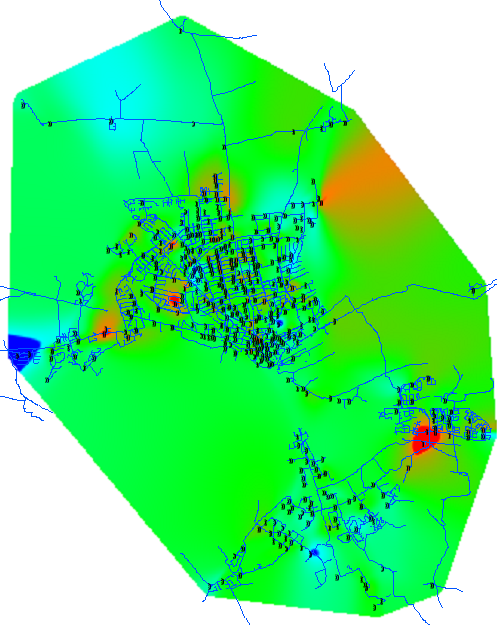
\includegraphics[width=0.55\textwidth]{report/pictures/fire_hydrants}
%\begin{tikzpicture}[scale=0.6,transform shape]

\begin{scope} [rotate around={0:(12,5.5)}, shift={(0.8,0)}]
\draw[thick,transform shape] (12,5.5) circle (0.5);
\draw[thick,transform shape] (12.5,5.5) -- (12,6);
\draw[thick,transform shape] (12.5,5.5) node (v1) {} -- (12,5);
\end{scope}

%man-valve
\begin{scope} [rotate ={-90}]
\node(n1) at (-5.25,16) {};
\draw[thick,transform shape](n1.center) -- ($(n1)-(0.5,0)$) --
($(n1)-(0,1)$) -- ($(n1)-(0.5,1)$) --  (n1.center);

\end{scope}

\draw [thick](15,5.5) -- (13.3,5.5);
\node at (15.5,6.2) {\large PRV};
\draw [thick](16,5.5) -- (17.5,5.5);
\draw [fill=cyan] [thick](9.1,5.7) -- (9.1,5.1) -- (10.9,5.1) -- (10.9,5.7);
\draw  [thick](9.1,6.1) -- (9.1,5.1) -- (10.9,5.1) -- (10.9,6.1);
\draw [thick](12.3,5.5) -- (10.9,5.5);
\end{tikzpicture} 
\caption{Difference calculation between observed and calculated pressures on fire hydrants\cite{verdo_doc}.}
\label{fig:pressure_mistakes}
\end{figure}

\vspace{-3mm}

\subsection{Grid balance and supply zones}
\label{grid_balance_supply_zones}

With the simulation model in EPANET there is a possibility to illustrate which pumping stations supply the different areas in the network. Simulations can be carried out for instance on supply areas in certain zones where more than one pumping station contributes to the consumption. The two zones, considered in this report are the HZ and LZ, in which the former is supplied by OMV and TBP and the latter is supplied by HBP and HSP where the tanks are placed on high elevation level. Consequently, as mentioned in \secref{waterworks_and_pumping_stations}, OMV and TBP are the waterworks and pumping stations which are responsible for filling the tanks in the HZ in HBP and HSP, respectively. 
Using the water quality properties of EPANET, a contamination was introduced first in OMV pumping station and then TBP. By introducing a contamination into the system, it can be tracked which parts of the network gets contaminated. \figref{fig:HSP_HBP_EPA} shows an example for this, illustrating the distribution between the two pumping stations, OMV and TBP. 


\begin{figure}[H]
\centering
\begin{subfigure}{.49\textwidth}
\centering
  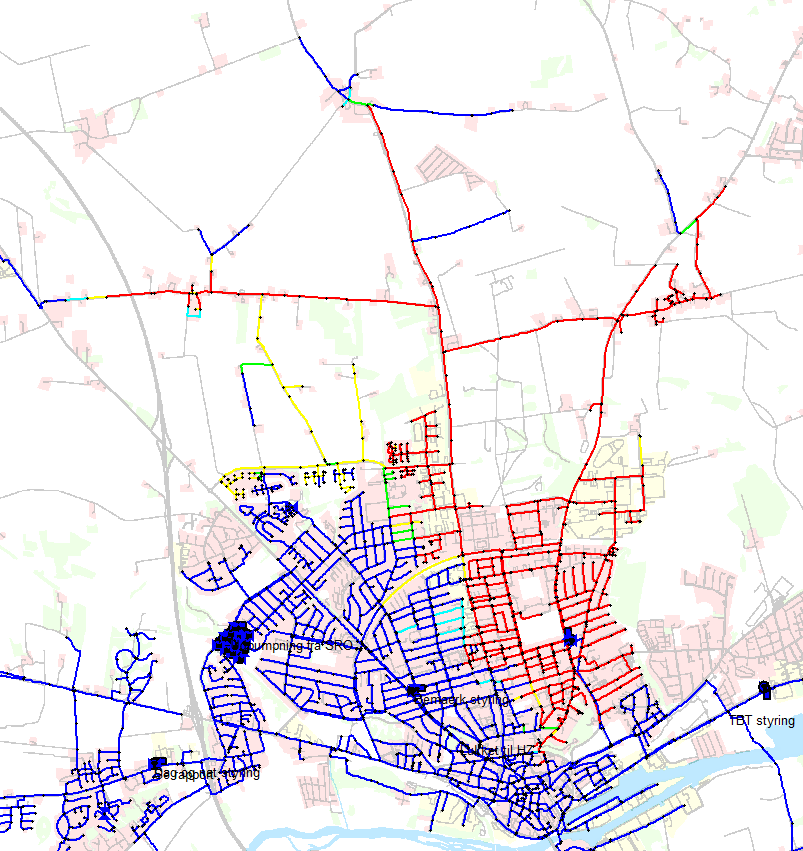
\includegraphics[width=0.75\textwidth]{report/pictures/HBP_HSP_distribution}
  \caption{HSP supply area, marked with red}
  \label{fig:HSP_HBP_EPA1}
\end{subfigure}
\begin{subfigure}{.49\textwidth}
\centering
  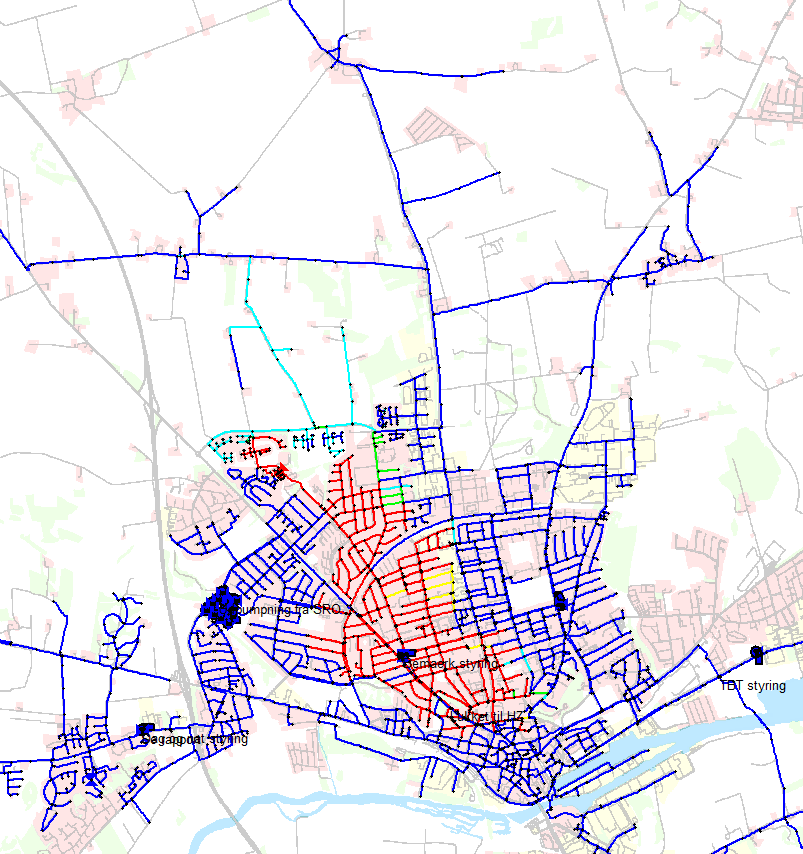
\includegraphics[width=0.75\textwidth]{report/pictures/HBP_HSP_distribution1}
  \caption{HBP supply area, marked with red}
  \label{fig:HSP_HBP_EPA2}
\end{subfigure}
\caption{Supply area by HSP(on the left) and supply area by HBP(on the right)\cite{verdo_doc}.}
\label{fig:HSP_HBP_EPA}
\end{figure}

\vspace{-3mm}

The red areas in \figref{fig:HSP_HBP_EPA} indicate 80-100 percent of drinking water originating from one or the other pumping station. However, the other colours(primarily yellow and green) indicate that there is a mix of water from both stations. The result in the grid is according to the control goals, as one pumping station supplies half of the region and an other the other one. This is achieved by controlling the flow in HBP and the pressure in HSP. 
